% ==================== 2.3.2.2 BCC ====================
\jiegou{2.3.2.2}{体心立方结构（BCC）}

体心立方（BCC）的演示对象是 $\alpha$-Fe，空间群与晶格常数等输入值见表~\ref{tab:bcc}。

\begin{table}[H]
  \centering
  \caption{体心立方（BCC）结构的建模参数}
  \label{tab:bcc}
  \begin{tabular}{ll}
    \toprule
    项目 & 参数 \\
    \midrule
    空间群 & $I\,m\,\bar3\,m$（No.~229） \\
    晶格常数 & $a=b=c=2.819$\,\AA，$\alpha=\beta=\gamma=90^\circ$ \\
    原子坐标 & Fe：$(0,0,0)$（$2a$ 位） \\
    化学式单元数 & $Z=2$ \\
    \bottomrule
  \end{tabular}
\end{table}

\begin{figure}[H]
  \centering
  \subcaptionbox{空间群与晶格常数设置}{%
    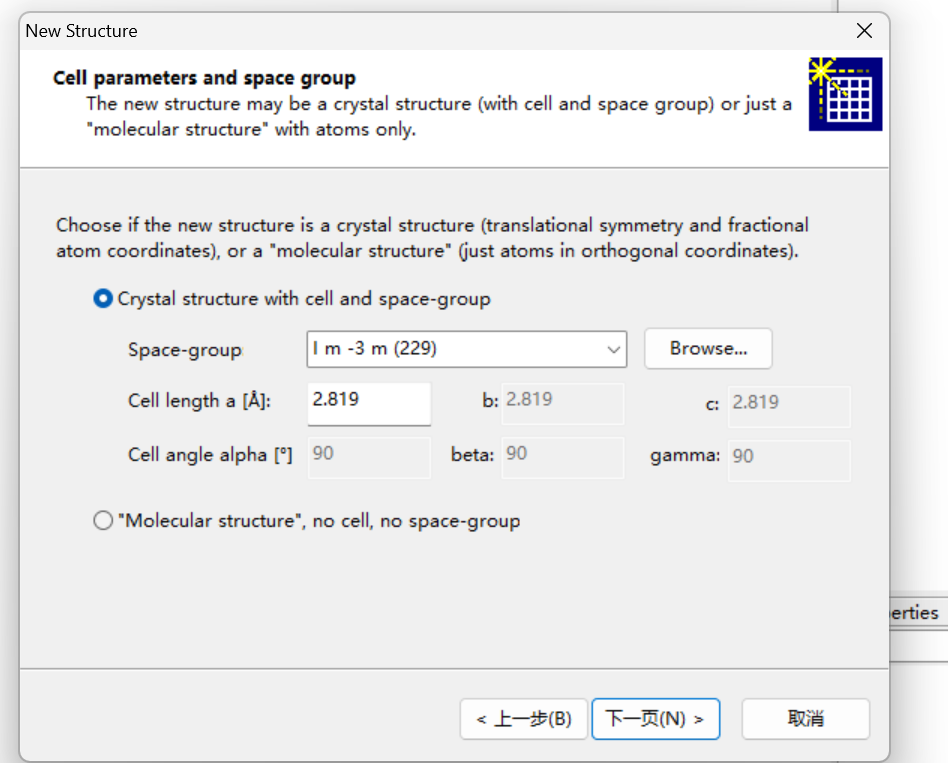
\includegraphics[width=0.44\textwidth]{assets/bcc/a.png}}
  \hfill
  \subcaptionbox{非对称单元原子（Fe）添加}{%
    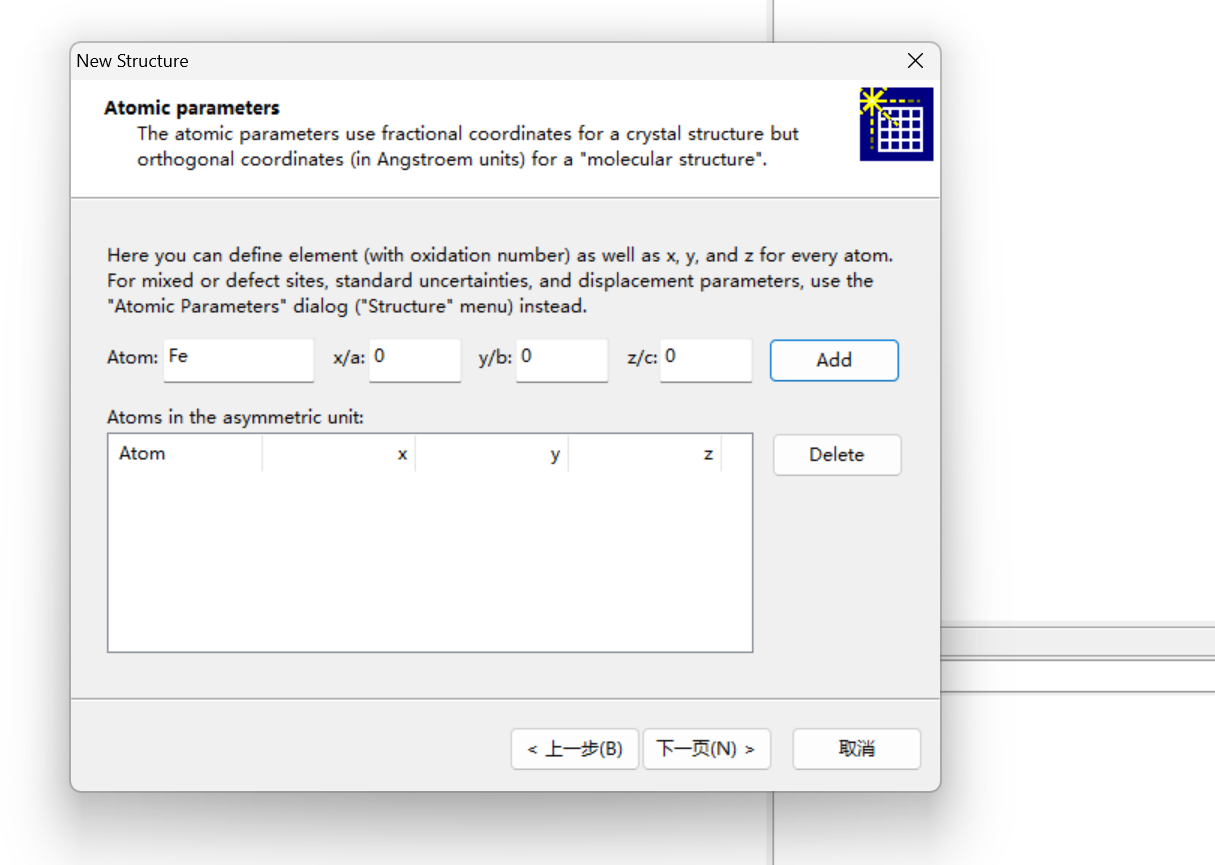
\includegraphics[width=0.44\textwidth]{assets/bcc/b.png}}
  \caption{体心立方（BCC）结构的参数设置}
  \label{fig:bcc-param}
\end{figure}

\begin{figure}[H]
  \centering
  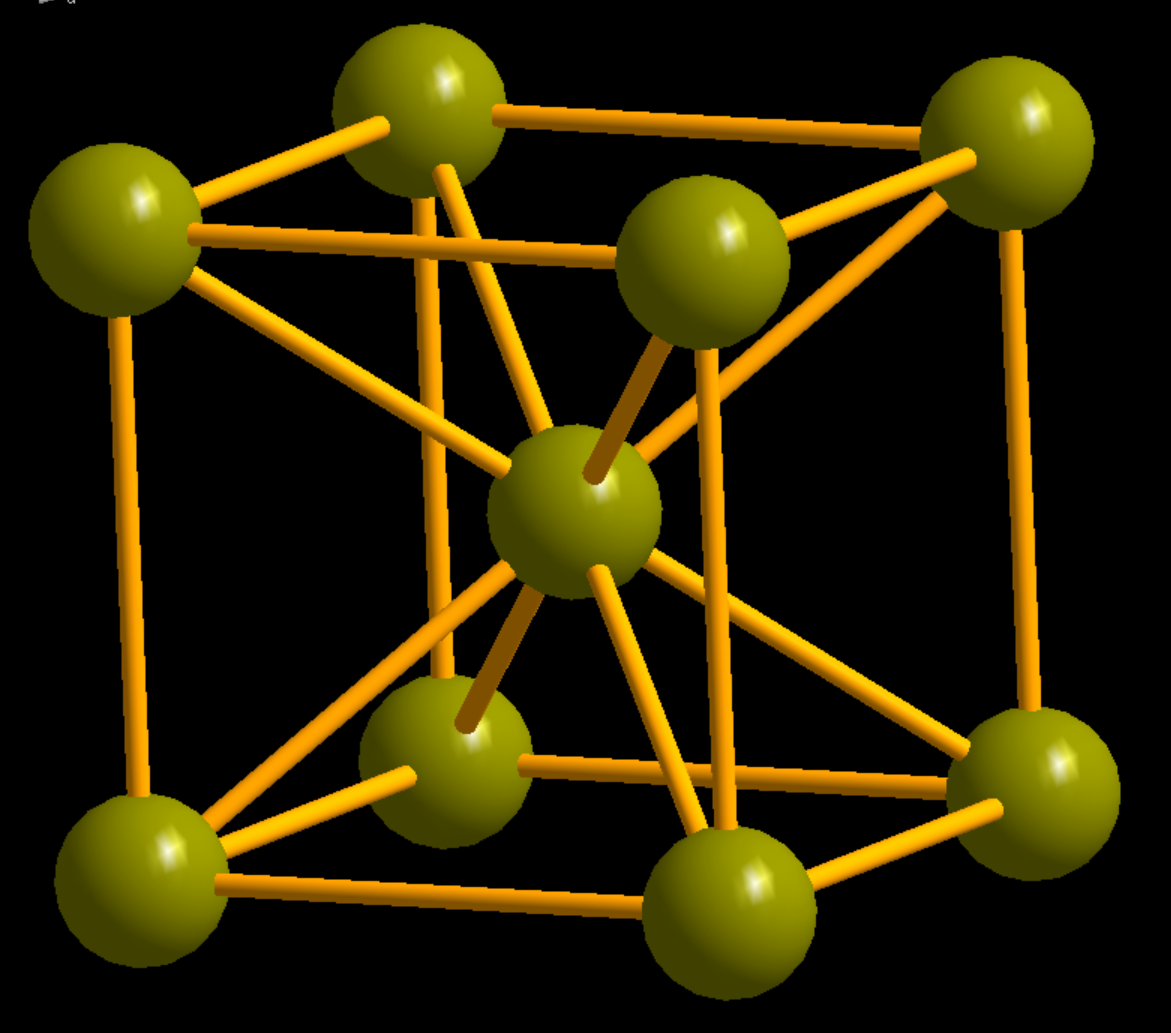
\includegraphics[width=0.5\textwidth]{assets/bcc/c.png}
  \caption{体心立方（BCC）结构的晶体结构模型}
  \label{fig:bcc-model}
\end{figure}

\begin{figure}[H]
  \centering
  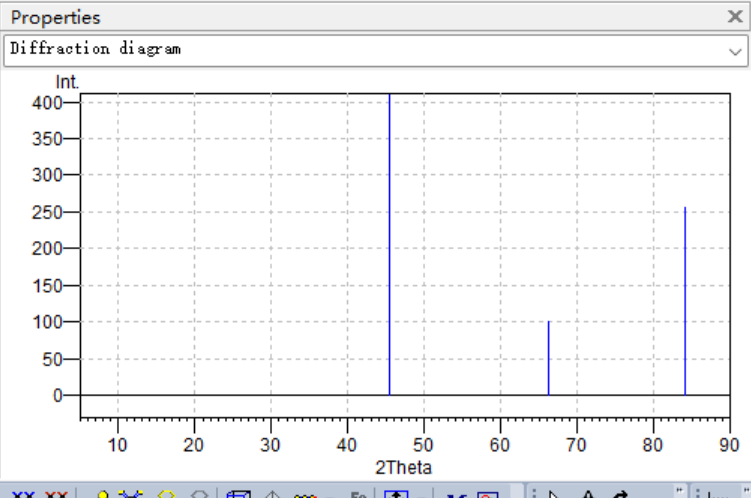
\includegraphics[width=0.5\textwidth]{assets/bcc/d.png}
  \caption{Diamond 模拟的体心立方（BCC）结构粉末衍射图}
  \label{fig:bcc-xrd}
\end{figure}

\begin{figure}[H]
  \centering
  \subcaptionbox{(111) 晶面视图}{%
    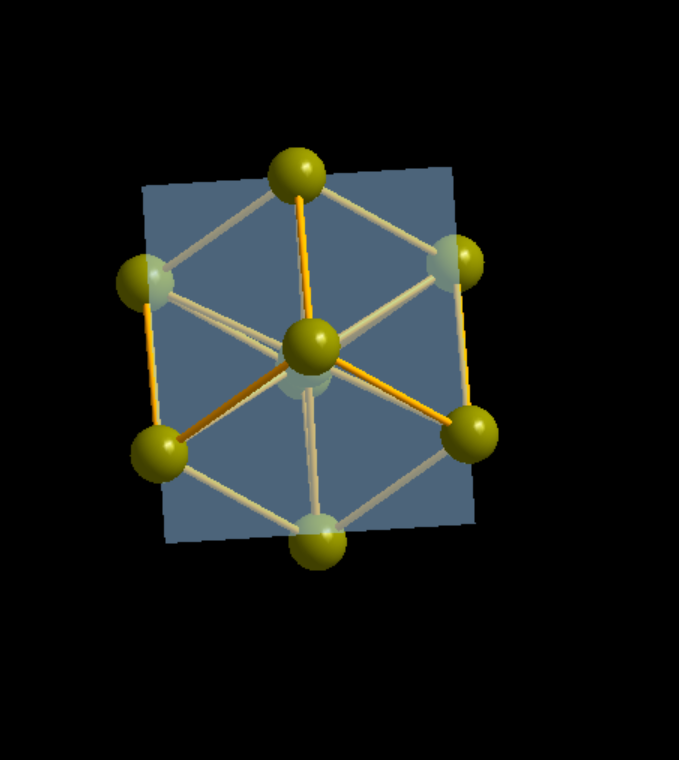
\includegraphics[width=0.44\textwidth]{assets/bcc/e.png}}
  \hfill
  \subcaptionbox{最近邻配位多面体（配位数 8）}{%
    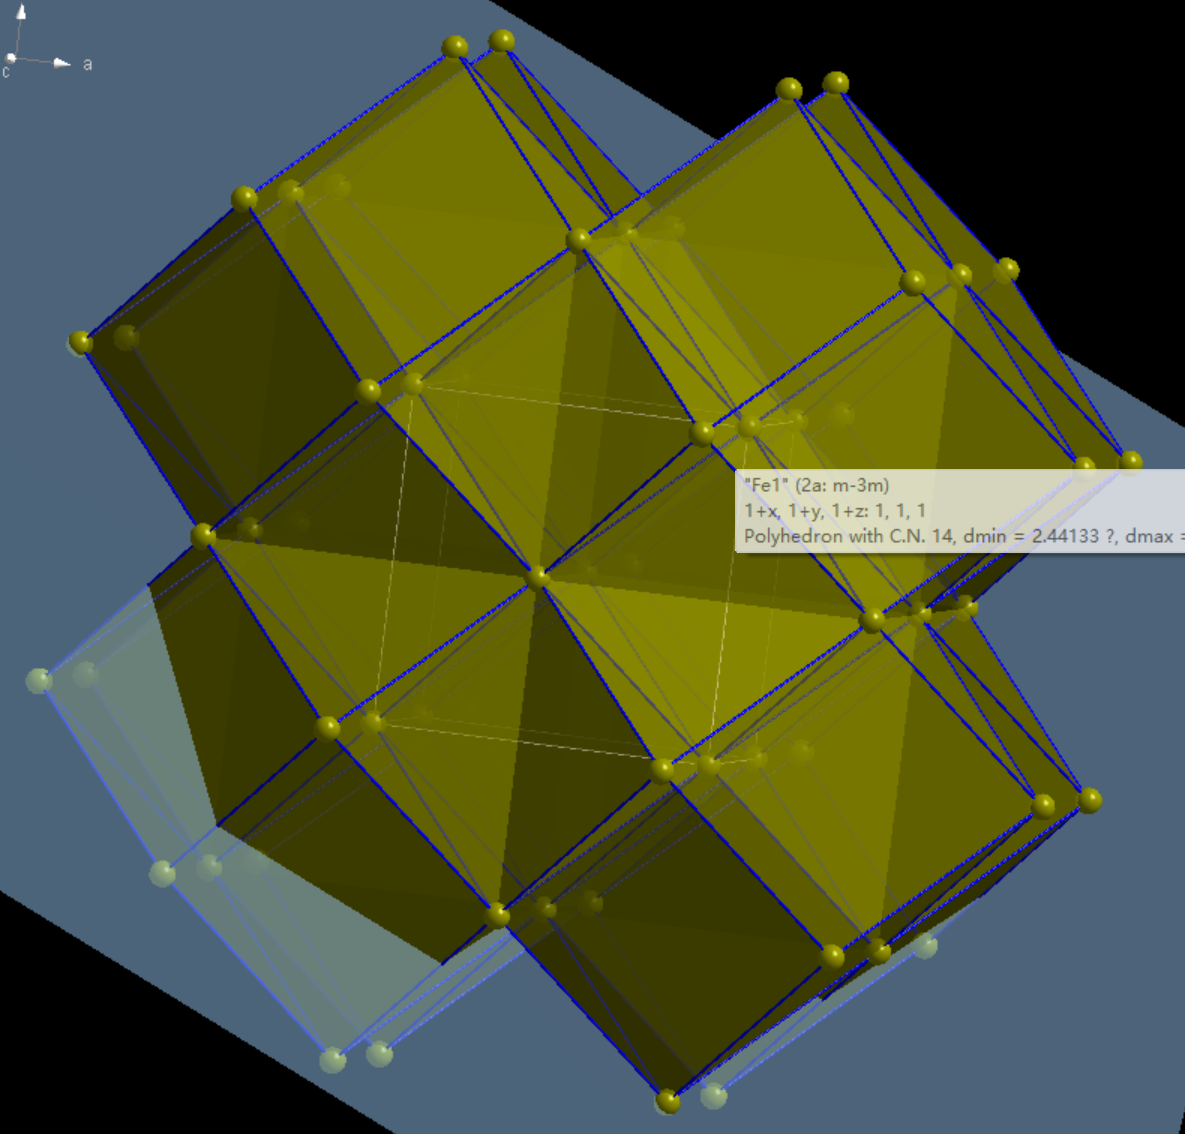
\includegraphics[width=0.46\textwidth]{assets/bcc/f.png}}
  \caption{体心立方（BCC）结构的晶面与配位多面体}
  \label{fig:bcc-plane}
\end{figure}

\textbf{结构特征。}顶点 8 个原子各计 $1/8$，再加上体心的 1 个，晶胞内共 2 个原子；
体心原子与 8 个顶点原子等距（图~\ref{fig:bcc-model}）。

沿体对角线方向，体心原子与两端的顶点原子相切，故 $4r=\sqrt{3}a$，$r=\sqrt{3}a/4$；
代入 $a=2.819$\,\AA 得 $r\approx1.22$\,\AA。最近邻 8 个，配位多面体为立方体
（图~\ref{fig:bcc-plane}(b)）；次近邻 6 个，位于 $\langle100\rangle$ 方向的相邻晶胞
体心。堆积因子为
\begin{equation}
  \eta=\frac{2\times\frac{4}{3}\pi r^3}{a^3}
    =\frac{2\times\frac{4}{3}\pi\left(\frac{\sqrt{3}}{4}a\right)^3}{a^3}
    =\frac{\sqrt{3}\pi}{8}\approx0.6802
\end{equation}
明显低于 FCC 与 HCP，$\alpha$-Fe 在相变（如马氏体相变）中伴随的体积变化正与此有关。
BCC 没有严格意义上的密排面，面间距最大的 $\{110\}$ 面可视为``最密''面；
图~\ref{fig:bcc-plane}(a) 演示的是在模型中添加 (111) 晶面（$d_{111}=1.6276$\,\AA）
后的观察效果。

$I\,m\,\bar3\,m$ 中的 $I$ 代表体心点阵，其余符号的含义与 FCC 相同。Cr、Mo、W、V 以及
碱金属 Na、K 等都是 BCC 结构，$\alpha$-Fe 是其中最熟悉的例子。
